\section{Hashing and Hash Function} \index{hashing}

Let $U$ be the universe of possible keys, and let $m$ be the size of the hash table. Then, we say that
$$
h:\; U \to \{0, \cdots, m-1 \}
$$
is a hash function.

If two keys are mapped to the same location/bucket/slot by the hash function, we say that they collide.

Furthermore, if $|U| > m$, then by the pigeonhole principle, there are at least two keys that collide. And because in virtually all cases, $|U| > m$, collision is unavoidable. A well-chosen hash function will minimize the number of collisions, but we still need some means to resolve collisions.

\begin{remark}
    A fun fact about the etymology of the word ``hash'': it is said that the word ``hash'' originated from the french word ``hache'', which refers to the action of chopping something into pieces. Hashing, as we will see, involves the same notion of randomly chopping and mixing.
\end{remark}

\section{Resolving Collision}

Chaining put all elements in $S \subseteq U$ that hash to the same slot in a linked list.

We define the load factor $\alpha$ to be $\alpha = n/m$ where $n = |S|$ and $m$ is the number of buckets (slots) in the hash table. $\alpha$ is the average number of elements of $S$ stored in a slot of the hash table.

Let $n_i$ be the number of elements of $S$ in slot $i$. Then,
$$
\sum_{i=0}^{m-1} n_i = n
$$

In the worst case, hashing with chaining takes $\Theta(\max_{0 \leq i \leq m-1} n_i)$ in addition to the time to compute $h(x)$ (the hashing step).

From the analysis above, we know that $\max\{n_i\} = n$ if all elements of $S$ map to the same bucket.

If $|U| > m(n-1)$, then by the pigeonhole principle, there exists $S \subseteq U$ with $|S|=n$ such that all element of $S$ hash to the same bucket.

Overall, hashing with chaining without randomization has the following time complexity:
\begin{itemize}
    \item $\proc{Insert}(x)$: $O(1)$ assuming all linked lists are unsorted and $x \not\in S$
    \item $\proc{Delete}(p)$: $O(1)$ if list is doubly linked; if singly linked, then $O(n_i)$ where $n_i$ is the size of the bucket where $p$ is in.
\end{itemize}

\section{Universal Hashing}

We can achieve better time complexity by randomly choosing the hash function. There is a family of hash functions that we call the universal hash functions, which we will define as follows.

\begin{definition}[Universal Hashing] \index{universal hashing}
    Let $\mathcal{H}$ be a finite collection of hash functions that map a given universe $U$ into the range $\{0,\cdots,m-1\}$. Such a collection is said to be universal if for each pair of distinct keys, $k,l \in U$, the number of hash functions $h \in \mathcal{H}$ for which $h(k) = h(l)$ is at most $|\mathcal{H}|/m$. In other words, with a hash function randomly chosen from $\mathcal{H}$, the chance of a collision between distinct keys is not more than the chance $1/m$ of a collision if $h(k)$ and $h(l)$ were randomly and independently chosen from the set $\{0,\cdots,m-1\}$.

    That is, a finite set $\mathcal{H}$ of hash functions from $U \to [0,\cdots,m-1]$ is universal if for all $x \neq y \in U$
    $$
    \Pr_{h \in \mathcal{H}} [h(x) = h(y)] \leq \frac{1}{m}
    $$
    or equivalently,
    $$
    \left| \{ h \in \mathcal{H} \mid h(x) = h(y) \} \right| \leq \frac{|\mathcal{H}|}{m}
    $$
\end{definition}

Here are some examples of universal hashing families.

\begin{enumerate}
    \item $\mathcal{H}$ is the set of all functions from $U \to [0,\cdots,m-1]$ assuming $U$ is finite. Let $u = |U|$. Then, $|\mathcal{H}|=m^u$. For any distinct $x,y\in U$
    $$
    \left| \{ h \in \mathcal{H} \mid h(x) = h(y) \} \right| = m^{u-1} = \frac{|\mathcal{H}|}{m}
    $$
    since there are $m$ choices for which bucket each element of $U - \{y\}$ gets mapped to. So,
    $$
    \Pr_{h \in \mathcal{H}} [h(x) = h(y)] = \frac{1}{m}
    $$
    Therefore, $\mathcal{H}$ is universal.

    \item Let $p$ be prime and $U = \{0,\cdots,p-1\} = \Z_p$. And let
    $$
    h_{a,b}(x) = [(ax+b) \bmod p] \bmod m
    $$
    and
    $$
    \mathcal{H}_{p,m} = \{h_{a,b}:\, U \to [0,\cdots,m-1] \mid a,b \in U, a \neq 0 \}
    $$
    So $|\mathcal{H}_{p,m}| = p(p-1)$. We can prove that $\mathcal{H}_{p,m}$ is universal.

    \item Let $U = \{0, \cdots, 2^k-1\}$ and let
    $$
    h_a(x) = \left\lfloor \frac{ax \bmod 2^k}{2^{k-m'}} \right\rfloor
    $$
    This selects the $(k-m'+1)$th through $k$th least significant bits. In other words, we throw away everything in $ax$ except the $k$ least significant bits, and then remove $k-m$ least significant bits. The size of the hash table is $m=2^{m'}$.
    
    Let
    $$
    \mathcal{H}' = \{ h_a \mid 0 < a < 2^k,\, \text{$a$ is odd}\}
    $$
    We have $|\mathcal{H}'| = u/2$. $\mathcal{H}'$ is universal. The proof is more complicated.
\end{enumerate}

For each of the universal hash families, let's also take a look at their sizes
\begin{enumerate}
    \item $|\mathcal{H}| = m^u$. To specify a hash function in $\mathcal{H}$, we need $u\log_2 m$ bits. This is too big.
    \item $|\mathcal{H}_{p,m}| < u^2$. To specify a hash function $\mathcal{H}_{p,m}$, we need less than $2 \log_2 u$ bits.
    \item $|\mathcal{H}'| = u / 2$. To specify a hash function in $\mathcal{H'}$, wee need $(\log_2 u) - 1$ bits.
\end{enumerate}

\section{Analysis of Hashing with Chaining}

Fix $S \subseteq U$ where $|S|=n$. Pick $h \in \mathcal{H}$ randomly where $\mathcal{H}$ is a universal family of hash functions from $U \to \{0,\cdots,m-1\}$.

Let $x \in U$. Let $C_x:\, \mathcal{H} \to \N$ be such that
$$
C_x(h) = \text{the number of keys in $S$ that hash to $h(x)$}
$$
$C_x$ is a random variable that depends on the choice of $h$.

For each $y \in S$, let $C_{x,y}:\; \mathcal{H} \to \{0,1\}$ be the indicator random variable that is $1$ if and only if $h(x)=h(y)$.
$$
C_x(h) = \sum_{y \in S} C_{x,y}(h)
$$

\begin{theorem}[Expected Number of Collisions For Each Key in Universal Hashing]
    $$
    \Expected_{h\in\mathcal{H}}[C_x] \leq 1+\frac{n}{m} = 1 + \alpha
    $$
\end{theorem}

\begin{proof}
    If $y=x$, then $C_{x,y}(h)=1$ for all $h \in \mathcal{H}$ so $\Expected_{h\in\mathcal{H}}[C_x] = 1$.

    If $y \neq x$, then
    $$
    \begin{aligned}
        \Expected_{h\in\mathcal{H}}[C_{x,y}] &= \Pr_{h\in\mathcal{H}}[C_{x,y}(h) = 1] & \text{since $C_{x,y}$ is indicator variable} \\
        &= \Pr_{h\in\mathcal{H}}[h(x)=h(y)] \leq 1/m & \text{since $\mathcal{H}$ is universal}
    \end{aligned}
    $$
    Hence,
    $$
    \begin{aligned}
        \Expected_{h\in\mathcal{H}}[C_x] &= \sum_{y\in S}\Expected_{h\in\mathcal{H}}[C_{x,y}] & \text{by linearity of expectation} \\
        &\leq 1 + \sum_{y \in S-\{x\}} \frac{1}{m} \leq 1 + \frac{n}{m} = 1+\alpha
    \end{aligned}
    $$
\end{proof}

\begin{corollary}
    The worst-case expected search time for $x$ is $O(1+\alpha)$.
\end{corollary}

\begin{corollary}
    Starting with an initially empty hash table of size $m$, the worst-case expected time to handle any sequence of $s$ \proc{Insert}, \proc{Delete}, \proc{Search} operations containing $n = O(m)$ \proc{Insert} operations is $O(s)$. Hence, we can perform each operation in $O(1)$ time.
\end{corollary}

\section{Perfect Hashing} \index{perfect hashing}

$h$ is perfect for $S$ if for each element of $S$ hashes to a different slot (i.e. no collisions). For example,
$$
h(x) = x \bmod 5
$$
is perfect for $\{1,14,20\}$, but not for $\{1,9,14\}$.

For a static dictionary (where $S$ does not change with no \proc{Insert} and \proc{Delete}),then it may be worthwhile to find a perfect hash function for $S$. For example, it is useful to construct a perfect hash function if we are designing a compiler for a programming language, and our $S$ is the set of reserved keywords in the language.

\subsection{Constructing a Perfect Hash Functions}

Let $S$ be a set of $n$ keys. Let $\mathcal{H}$ be a universal family of hash functions. Let $C:\, \mathcal{H}\to\N$ be the random variable so that
$$
C(h) = \text{the number of collisions when $h$ is used to hash $S$}
$$
More formally,
$$
C(h) = \left| C_{x,y} \in S \mid x \neq y,\, h(x)=h(y) \right|
$$
where $C_{x,y}$ is defined similarly as the indicator variable that is $1$ if and only if $h(x)=h(y)$. 

\begin{lemma}[Expected Number of Collisions in Universal Hashing]
    $$
    \Expected[C] \leq \frac{{n \choose 2}}{m}
    $$
\end{lemma}

\begin{proof}
    $$C(h) = \sum \{ C_{x,y}(h) \mid x<y,\, x,y \in S \}$$
    By linearity of expectation,
    $$
    \begin{aligned}
        \Expected_{h \in \mathcal{H}} [C] &= \sum \{ \Expected_{h \in \mathcal{H} } [C_{x,y}] \mid x,y \in S,\, x < y\} \\
        &= \sum \{ \Pr_{h \in \mathcal{H}} [h(x)=h(y)] \mid x,y\in S,\, x<y\} \\
        &\leq \sum \{1/m \mid x,y \in S,\, x<y \} & \text{since $\mathcal{H}$ is universal} \\
        &= \frac{{n \choose 2}}{m} & \text{since there are ${n \choose 2}$ pairs of keys that may collide}
    \end{aligned}
    $$
\end{proof}

If $m > {n \choose 2}$, then $\Expected_{h \in \mathcal{H}}[C] < 1$. Since $C(h) \in \N$ for all $h \in \mathcal{H}$, this implies that there exists some $h \in \mathcal{H}$ such that $C(h) = 0$. This tells if we are willing to use $\Theta(n^2)$ space for the hash table, there exists a hash function $h \in \mathcal{H}$ that is perfect for $S$, so that \proc{Search} only takes only one step.

\begin{theorem}
    If $m > 2 {n \choose 2} = n(n-1)$, then
    $$
    \Expected_{h \in \mathcal{H}}[C] < \frac{1}{2}
    $$
    This means more than half of the functions in $\mathcal{H}$ is perfect for $S$.
\end{theorem}

The randomized algorithm for constructing a perfect hash function, we

\begin{codebox}
    \Procname{$\proc{Construct-Perfect-Hash}(\mathcal{H}, S)$}
    \li Pick $h \in \mathcal{H}$ uniformly at random.
    \li \For $s$ in $S$ \Do
        \li \If there is a collision \Then
        \li start over and try again
    \End \End
    \li \If no collision \Then
        \li \Return $h$ 
\end{codebox}

If $m > 2 {n \choose 2}$, the expected number of tries is less than 2, and the algorithm takes $O(2n)$ time to find a perfect hash function for $S$.

\subsection{FKS Hashing} \index{FKS hashing}

However, sometimes when the size of $S$ is large, the $O(n^2)$ space that our current perfect hashing table is not longer ideal. In this case, we want to use $m \in O(n)$ space for the hash table. Then,
$$
\Expected[C] = \frac{{n \choose 2}}{m} \in O(n)
$$
Some buckets will have size $>1$, but all buckets are likely to have size $O(\sqrt{n})$. Essentially, if a bucket have size $b$, there are at least $\displaystyle {b \choose 2}$ collisions. 

The idea is to use a perfect hash function to represent each bucket. If the size of bucket $i$ is $b$, we will use $b^2$ space for it. The resulting data structure is a 2-level hash. For $i=0,\cdots,m-1$, let $n_i(h) = \{ x \in S \mid h(x_i) = i \}$ be the number of keys in $S$ that get mapped to bucket $i$ by $h$. An example of the resulting hash table is shown in Figure \ref{fig:fks-hashing}.

$$
\sum_{i=0}^{m-1} n_i(h) = n
$$

\begin{figure}[htbp]
    \centering
    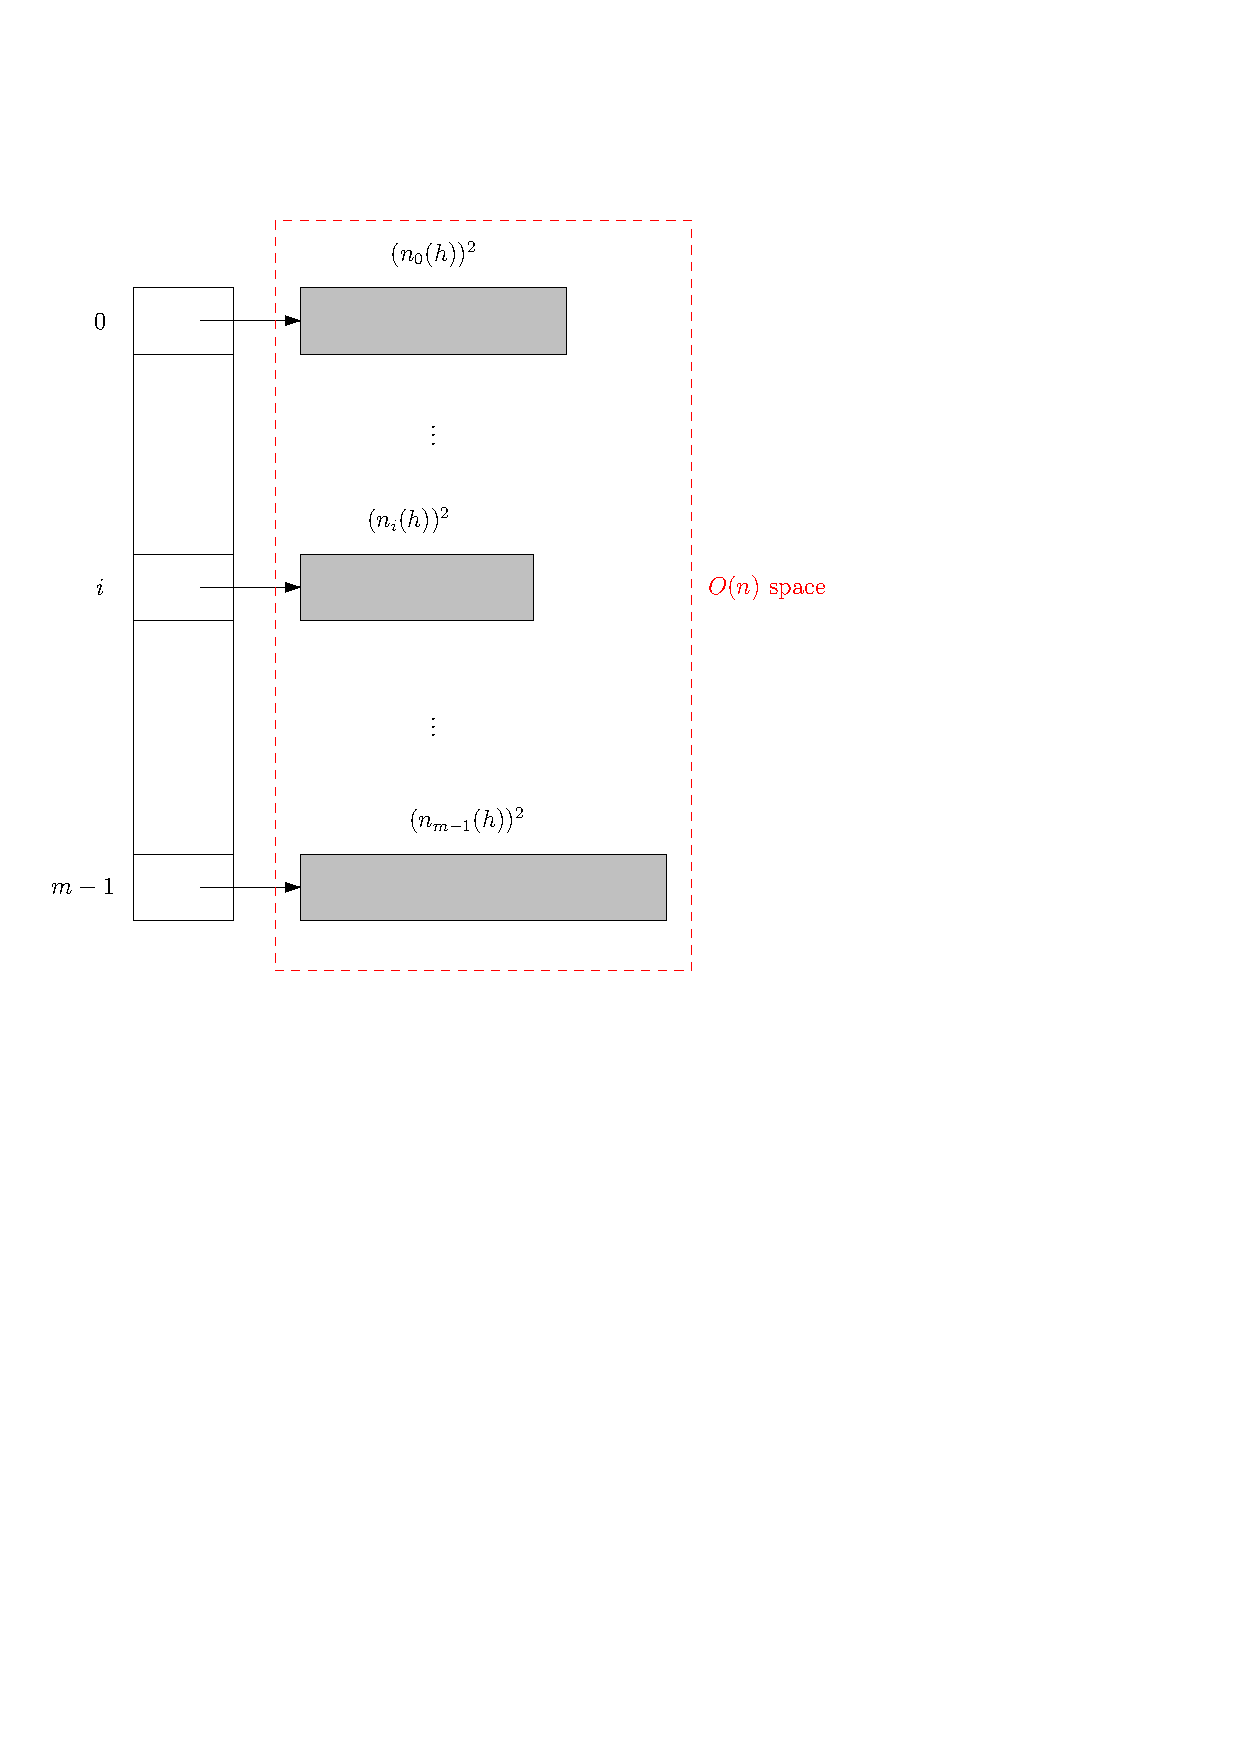
\includegraphics[width=0.5\linewidth]{fks-hashing.pdf}
    \vspace{2em}
    \caption{FKS 2-level hash table. As shown in the diagram and explained above, the length of each secondary hash table is $(n_i(h))^2$. }
    \label{fig:fks-hashing}
\end{figure}

The expected amount of space used by all the secondary hash tables can be computed as follows:

$$
\begin{aligned}
    C(h) &= \sum_{i=0}^{m-1} {n_i(h) \choose 2} \\
    &= \sum_{i=0}^{m-1} \frac{n_i(h)^2}{2} - \sum_{i=0}^{m-1} \frac{n_i(h)}{2} \\
    &= \frac{1}{2} \sum_{i=0}^{m-1} n_i(h)^2 - \frac{n}{2}
\end{aligned}
$$
By linearity of expectation,
$$
\begin{aligned}
    \Expected\left[ \sum_{i=0}^{m-1} n_i(h)^2 \right] &= 2 \Expected[C] + n \\
    &= 2\frac{{n \choose 2}}{m} + n \in \Theta(n) & \text{if $m \in \Theta(n)$ }
\end{aligned}
$$

$h$ itself is not a perfect hash function. For each non-empty bucket, find a hash function $h_i:\; U \to \{0,\cdots,m_i-1\}$, where $m_i = (n_i(h))^2$, that is perfect for the seconday hash table at bucket $i$ (i.e. perfect for the set $\{ x \in S \mid h(x) = i \}$).

\subsection{Representing FKS Hash Table}

In practice, we can represent the two-level FKS hash table for $S \subseteq U$ as a single array. Suppose that $U = \{ 0, \cdots, p-1 \}$. We use $\mathcal{H}_{p,m}$ for different values of $m$.

The first 3 locations of the array contain $m$, $a$, and $b$ used to specify the first-level hash function $h$. In particular, $m$ is the size of the first-level hash table; $a$ and $b$ are the parameters for the first-level table.

The next $m$ locations contain pointers to array corresponding to each second-level hash table.

Each second-level table is stored preceeded by the specifications of its hash function: $m_i = n_{i}(h_{a,b})$ and the parameter $a_i + b_i$ that specifies the perfect hash function $h_{a_i,b_i}$ for the $i$th secondary hahs table.

\begin{example}
    Let $p=31$. $U= \{0,\cdots,30\}$, $n=6$, and $S= \{2,4,5,15,18,30\}$, so $n=6$. Let the size of the first-level hash table be $m$.

    We randomly choose a hash function from $\mathcal{H}_{31,6}$ for the first-level table. Suppose that we end up getting
    $$
    h_{2,0}(x) = [(2x+0) \bmod 31] \bmod 6
    $$
    as the hash function.

    In this case,
    \begin{itemize}
        \item Bucket 0 contains: 15; so $n_0(h)=1$ and  $n_0(h)^2=1$,
        \item Bucket 2 contains: 4; so $n_2(h)=1$ and $n_2(h)^2=1$,
        \item Bucket 4 contains: 2, 5; so $n_4(h)=2$ and $n_4(h)^2=4$,
        \item Bucket 5 contains: 18, 30; so $n_5(h)=2$ and $n_5(h)^2=4$, and
        \item All other buckets are empty with $n(h) = 0$.
    \end{itemize}

    The two-level hash table would looks like Figure \ref{fig:fks-hashing-example}
    \begin{figure}[htbp]
        \centering
        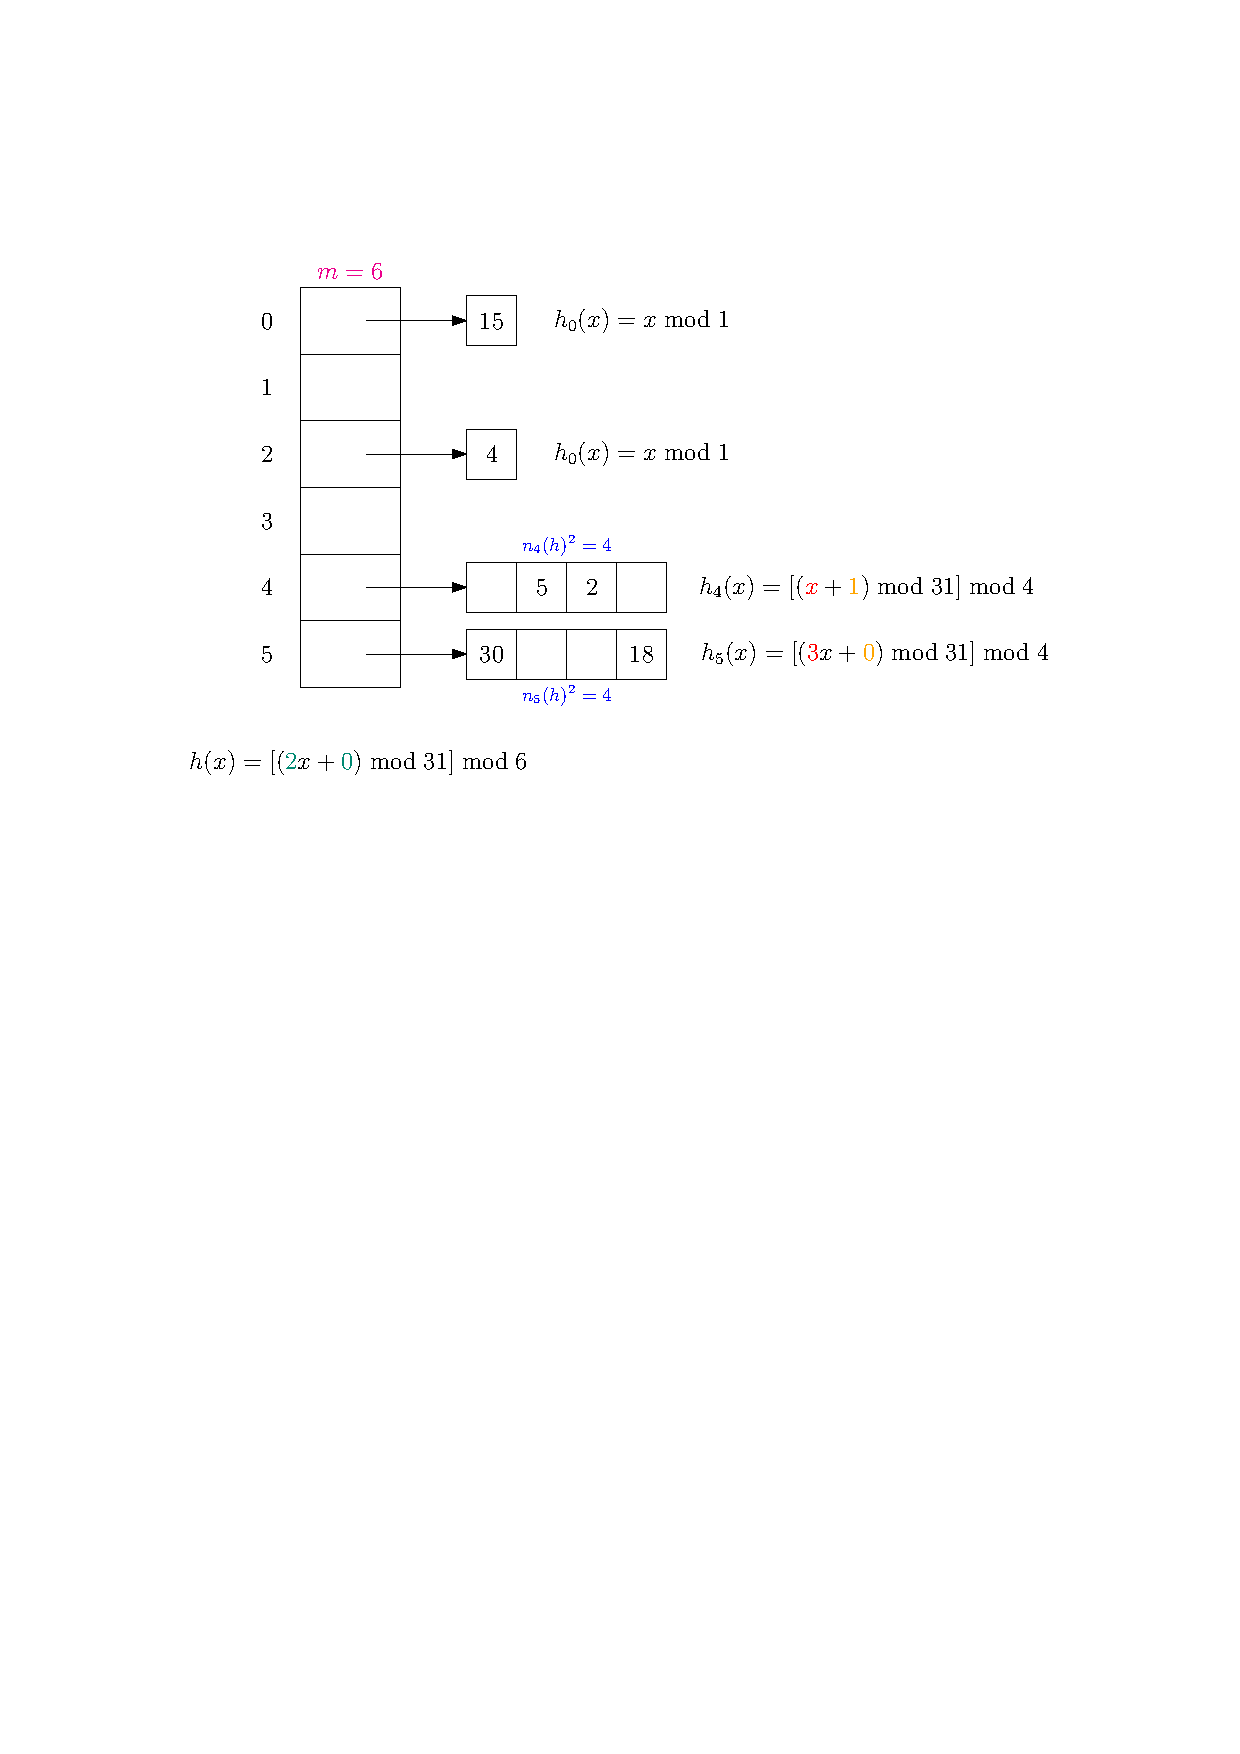
\includegraphics[width=0.6\linewidth]{fks-hashing-example.pdf}
        \caption{Example of a two-level hash table}
        \label{fig:fks-hashing-example}
    \end{figure}

    If we were to represent this two-level using a 1-D array, it should look like Figure \ref{fig:fks-hashing-example-array}
    \begin{figure}[htbp]
        \centering
        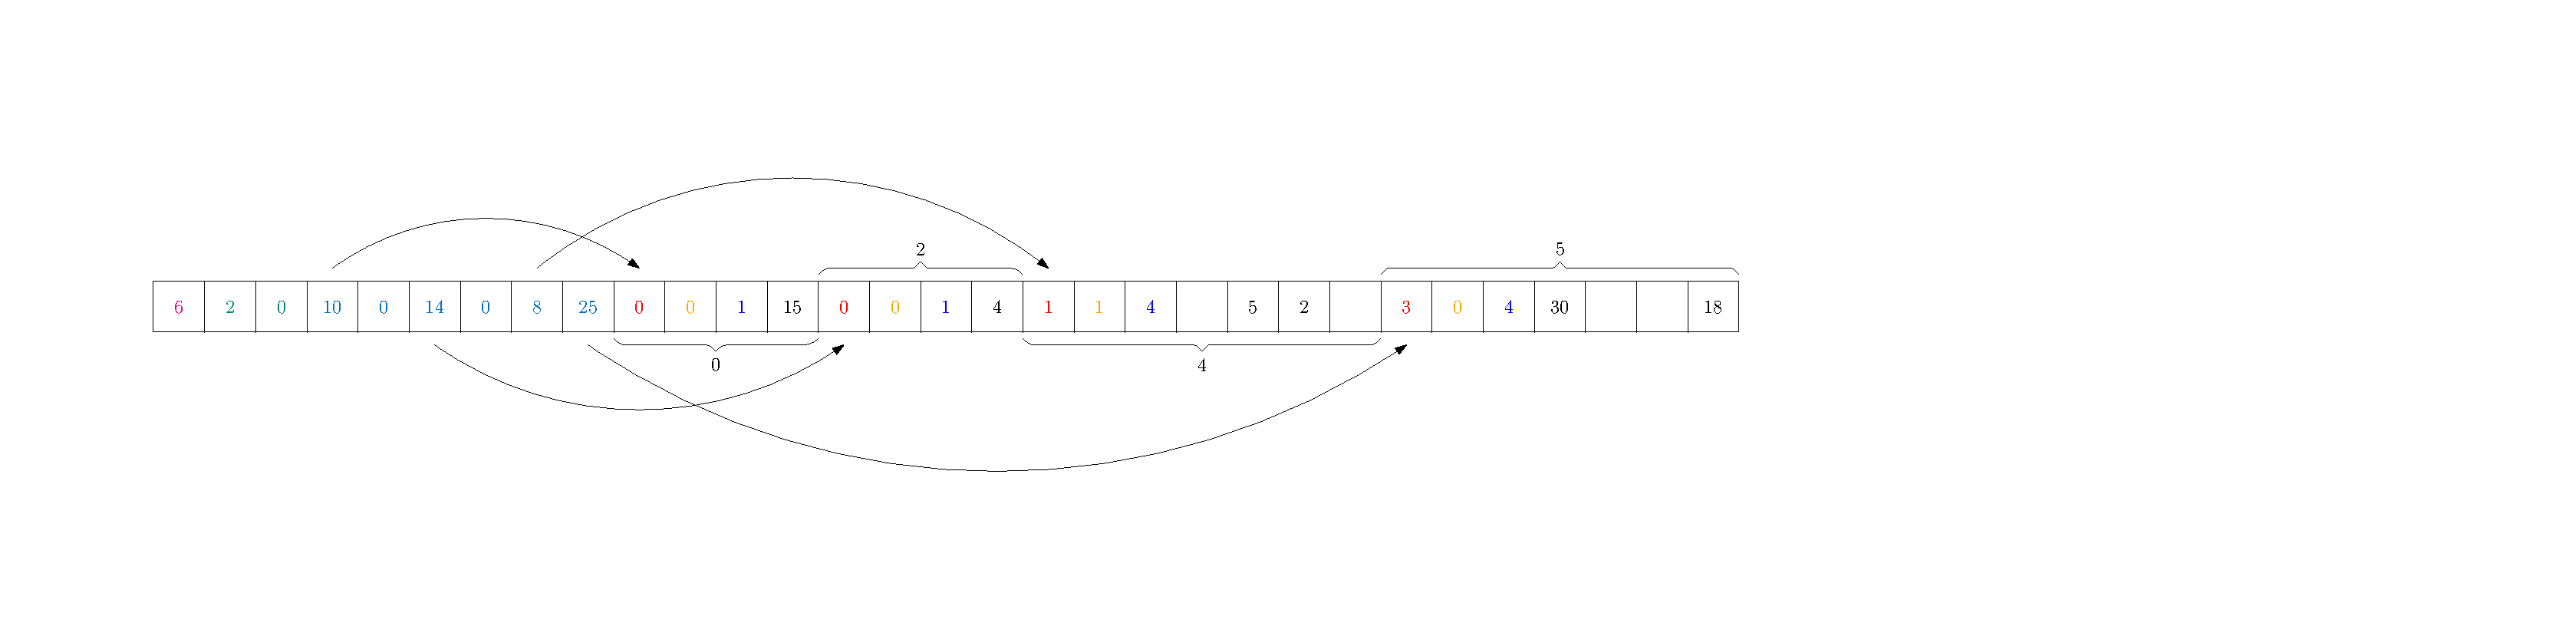
\includegraphics[width=\linewidth]{fks-hashing-example-array.pdf}
        \caption{The previous two-level hash table represented by an array. The colored represents the corresponding parameters in the two-level hash table representation.}
        \label{fig:fks-hashing-example-array}
    \end{figure}
\end{example}

\pagebreak

\begin{remark}
    This two-level hash table is often called the FKS hash table, which owes its name to its inventors M. Fredman, J. Koml\'{o}s, and E. Szemer\'{e}di. They published the article titled \href{https://www.cs.dartmouth.edu/~ac/Teach/CS105-Winter05/Handouts/fks-perfecthash.pdf}{\textit{Storing a Sparse Table with O(1) Worst Case Access Time}} in 1984, in which they first introduced this kind of hash table.
\end{remark}

\section{Open Addressing} \index{open addressing} \index{linear probing}

The idea of open addressing is to store keys directly into the hash table. If the hash table is full, we cannot insert new elements, unless we create a new hash table and double the size. In open addressing, rather than mapping each key to a single slot and use chaning to resolve collision, we instead compute a sequence of slots. With such approach, the load factor $\alpha$ can never exceed 1.

Let $h:\; U \times \{0,\cdots,m-1\} \to \{0,\cdots,m-1\}$. For each key $k_1$, its probe sequence 
$$
(h(k,0), h(k,1),\cdots, h(k,m-1))
$$
is a permutation of $(0,1,\cdots,m-1)$ 

For $\proc{Insert}(H,k)$, we put $k$ into the first empty $(N_i)$ slot in its probe sequence.

\section{Application of Hashing}

Given an array $A$ of $n$ numbers, determine if all of them are different.

\begin{itemize}
    \item Sort the array and then check if adjacent numbers are duplicates. The time complexity would be $O(n\log n + n)$, where the $n\log n$ is from sorting the array and $n$ is for iterating over the array.
    \item Insert every element into the hash table on at a time. Each time, check for duplicates with a search. This take $\Theta(n)$ worst-case expected time.
\end{itemize}

Given a list of $n$ possible integers $x_1,x_2,\cdots,x_n$, determine in $O(n)$ worst-case expected time if there exists and $i$ and $j$ such that $x_i = x_j + 1$.